\block{Recognition System}{
	\section*{Overview}
	Fig. 2 presents the main processing stages of the implemented banknote recognition system. The C++ source code along with the complete results are available at \url{https://github.com/carlosmccosta/Currency-Recognition}.

	\centering
	\begin{minipage}[t]{.66\linewidth}
		\begin{tikzfigure}
			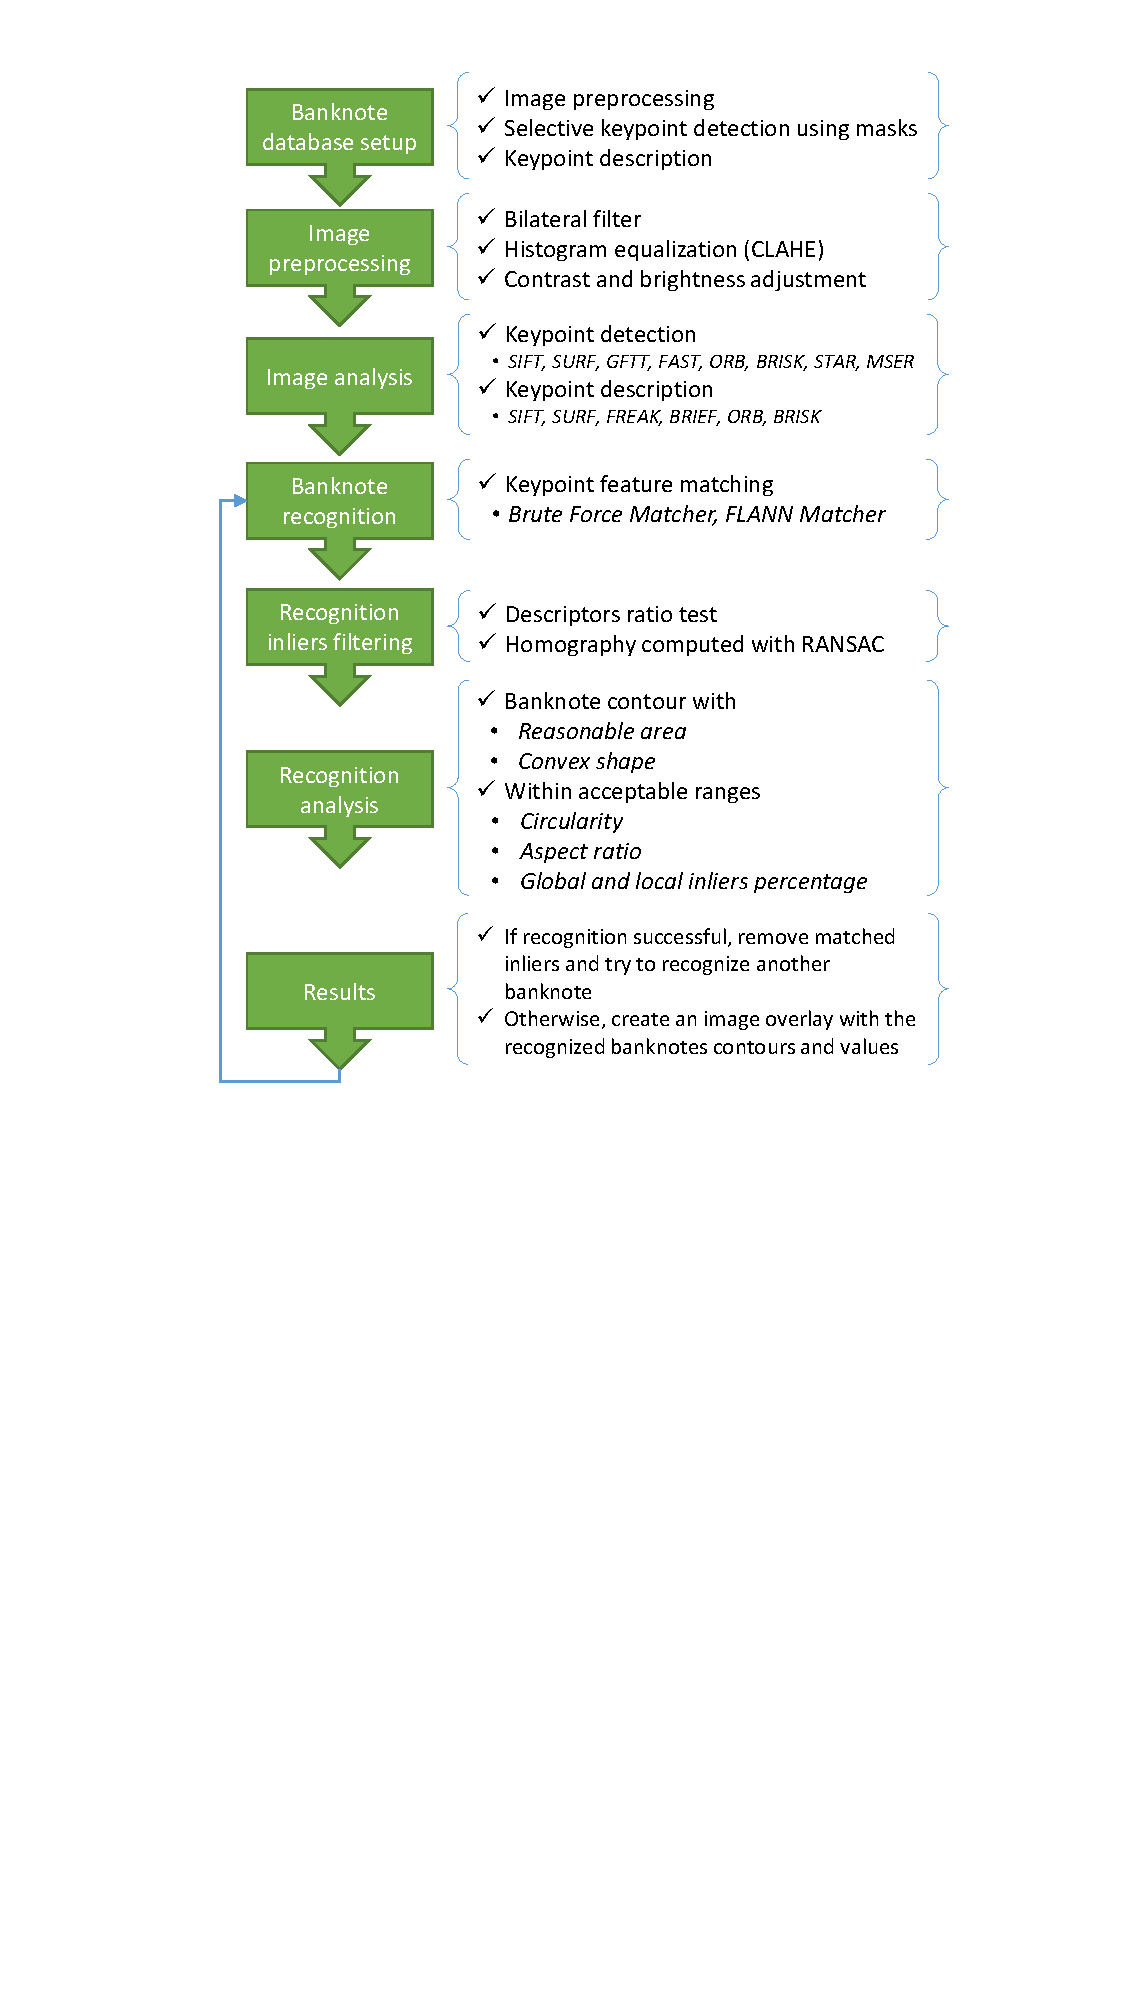
\includegraphics[width=\linewidth]{system-overview}
			\captionof{figure}{Overview of main processing modules}
		\end{tikzfigure}
	\end{minipage}
	\begin{minipage}[t]{.33\linewidth}
		\begin{tikzfigure}
			\centering

			\vspace*{.37em}
			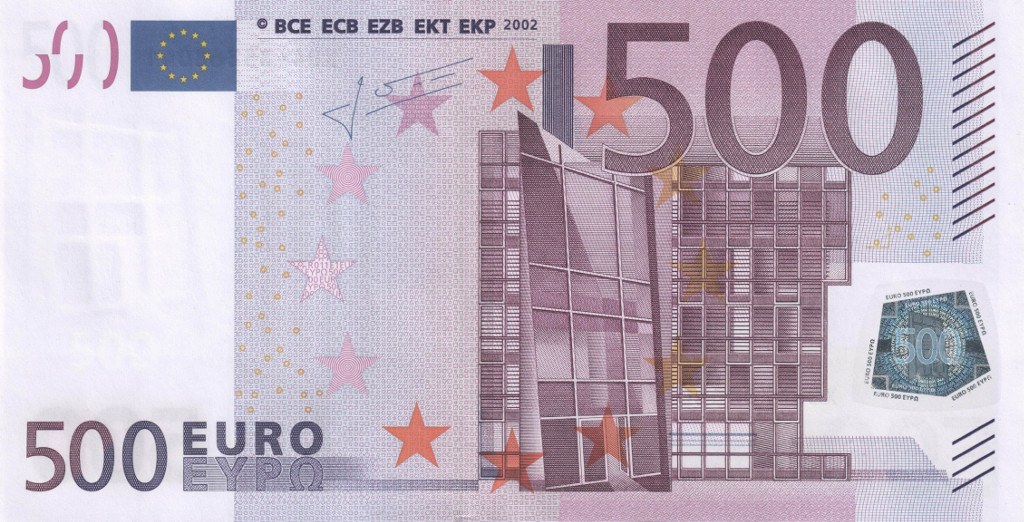
\includegraphics[width=.485\linewidth]{notes-masks/500eu-front}
			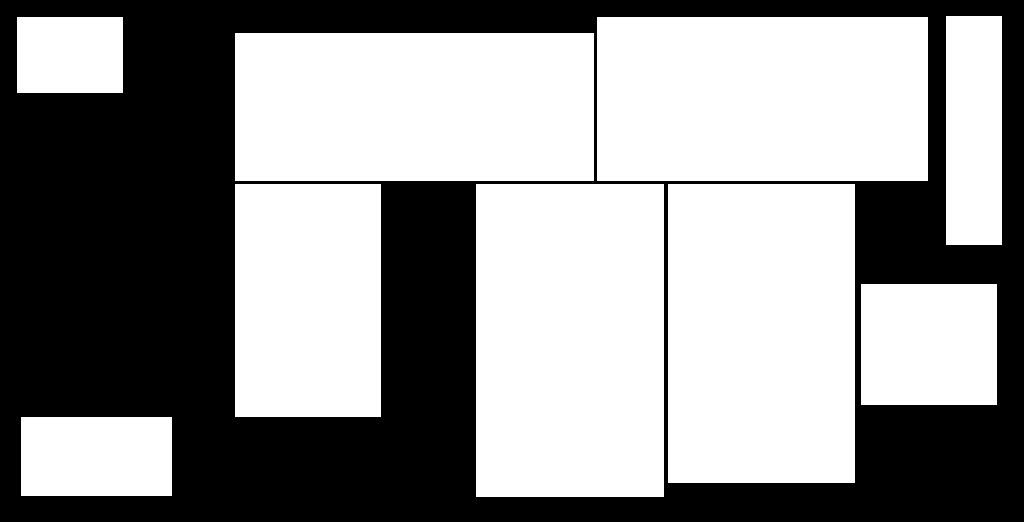
\includegraphics[width=.485\linewidth]{notes-masks/500eu-front-mask}

			\vspace*{0.8em}
			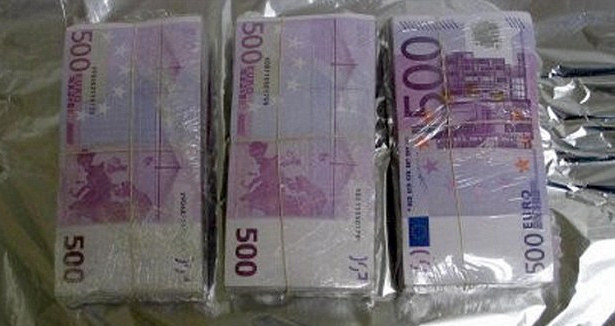
\includegraphics[width=.485\textwidth]{preprocessing/500-500-500}
			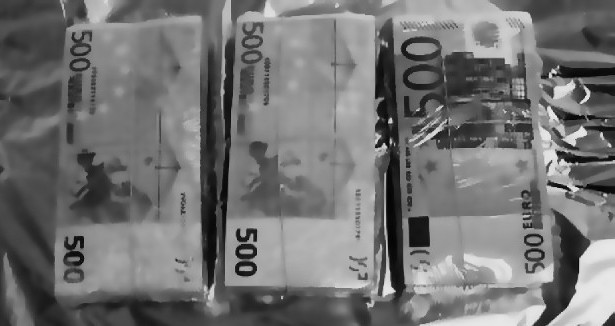
\includegraphics[width=.485\textwidth]{preprocessing/500-500-500-preprocessed}

			\vspace*{1.2em}
			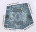
\includegraphics[width=.2496\textwidth]{image-resolution/500eu-front-very-low}\hfill
			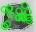
\includegraphics[width=.2496\textwidth]{image-resolution/500eu_front_currencyDB_veryLowResolution_SIFT-Detector}\hfill
			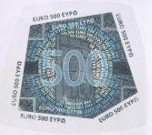
\includegraphics[width=.2499\textwidth]{image-resolution/500eu-front-medium}\hfill
			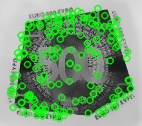
\includegraphics[width=.2499\textwidth]{image-resolution/500eu_front_currencyDB_mediumResolution_SIFT-Detector}

			\vspace*{.9em}
			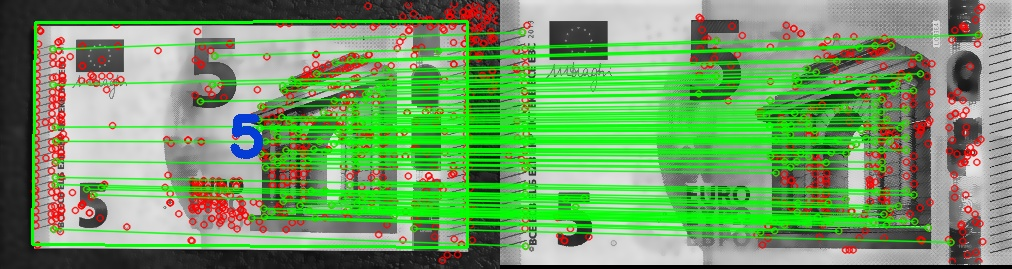
\includegraphics[width=.99\textwidth]{notes-recognition/5__(5).jpg___SIFT-Detector_SIFT-Extractor_BF-Matcher_lowQualityImageDB_globalMatch__inliersMatches__0}
			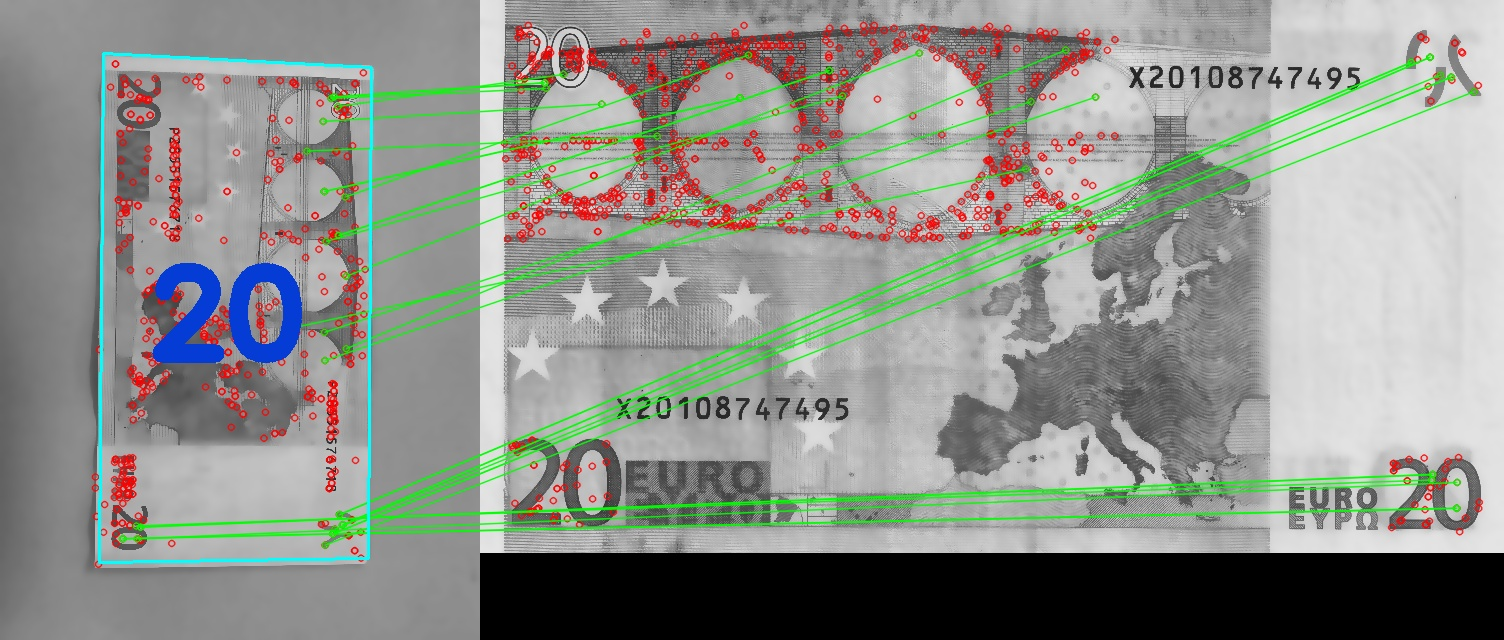
\includegraphics[width=.8\textwidth]{notes-recognition/20__(13).jpg___SIFT-Detector_SIFT-Extractor_BF-Matcher_mediumQualityImageDB_globalMatch__inliersMatches__0}

			\vspace*{.8em}
			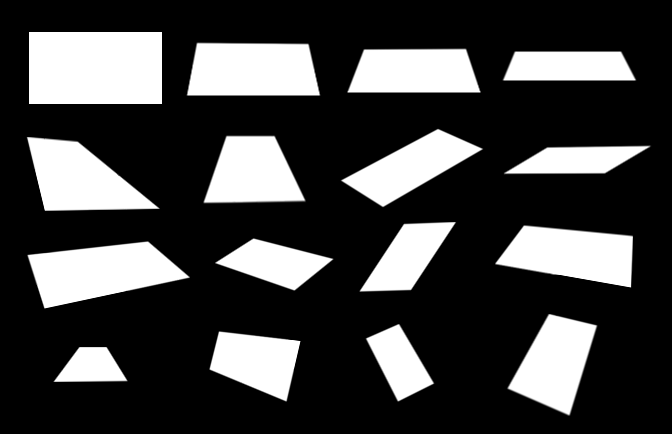
\includegraphics[width=0.75\textwidth]{notes-masks/currency-db-shapes}

			\vspace*{.5em}
			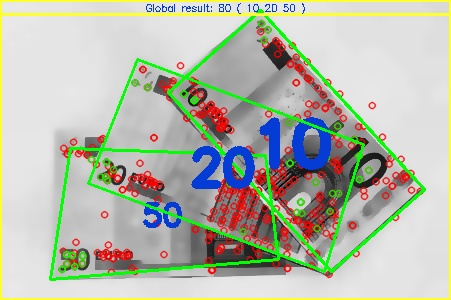
\includegraphics[width=0.8\textwidth]{notes-recognition/10-20-50.jpg___SIFT-Detector_SIFT-Extractor_BF-Matcher_dynamicQualityImageDB_globalMatch}
		\end{tikzfigure}
	\end{minipage}
}
